\section{Persiapan}
\subsection{Instalasi Java}
\subsection{Instalasi Android Studio}
\begin{enumerate}
	\item Kemudian klik dua kali pada installer yang telah di-download untuk memulai proses instalasi. Installer akan menampilkan Android Studio Setup seperti gambar berikut, lalu klik Next. 
	\begin{figure}[H]
		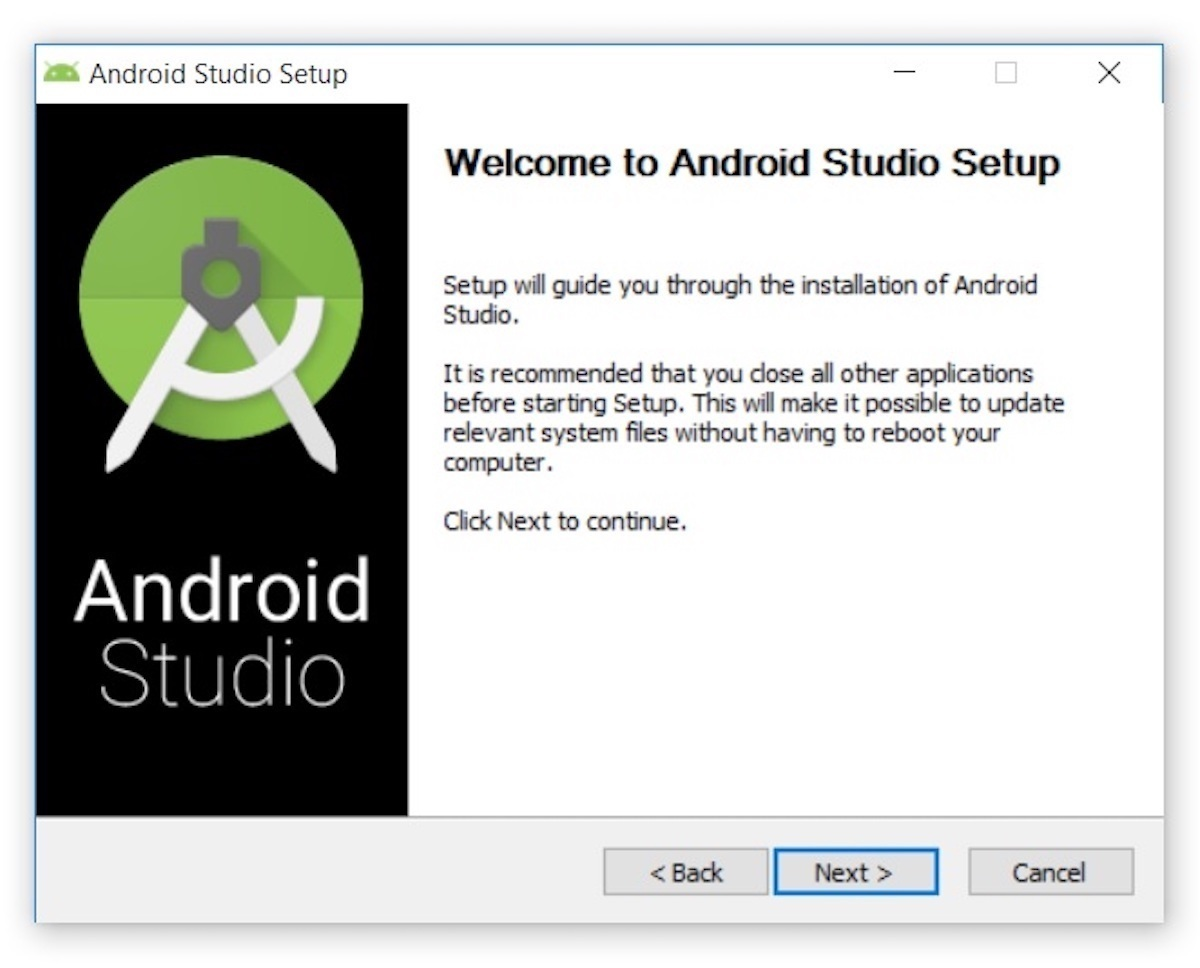
\includegraphics[width=4cm]{figures/installas/1.jpg}
		\centering
		\caption{Android Studio Setup.}
	\end{figure}
	\item Setelah itu kita diberi opsi untuk menginstal Android Virtual Device. Disini kita biarkan default setting-nya, lalu klik Next.
	\begin{figure}[H]
		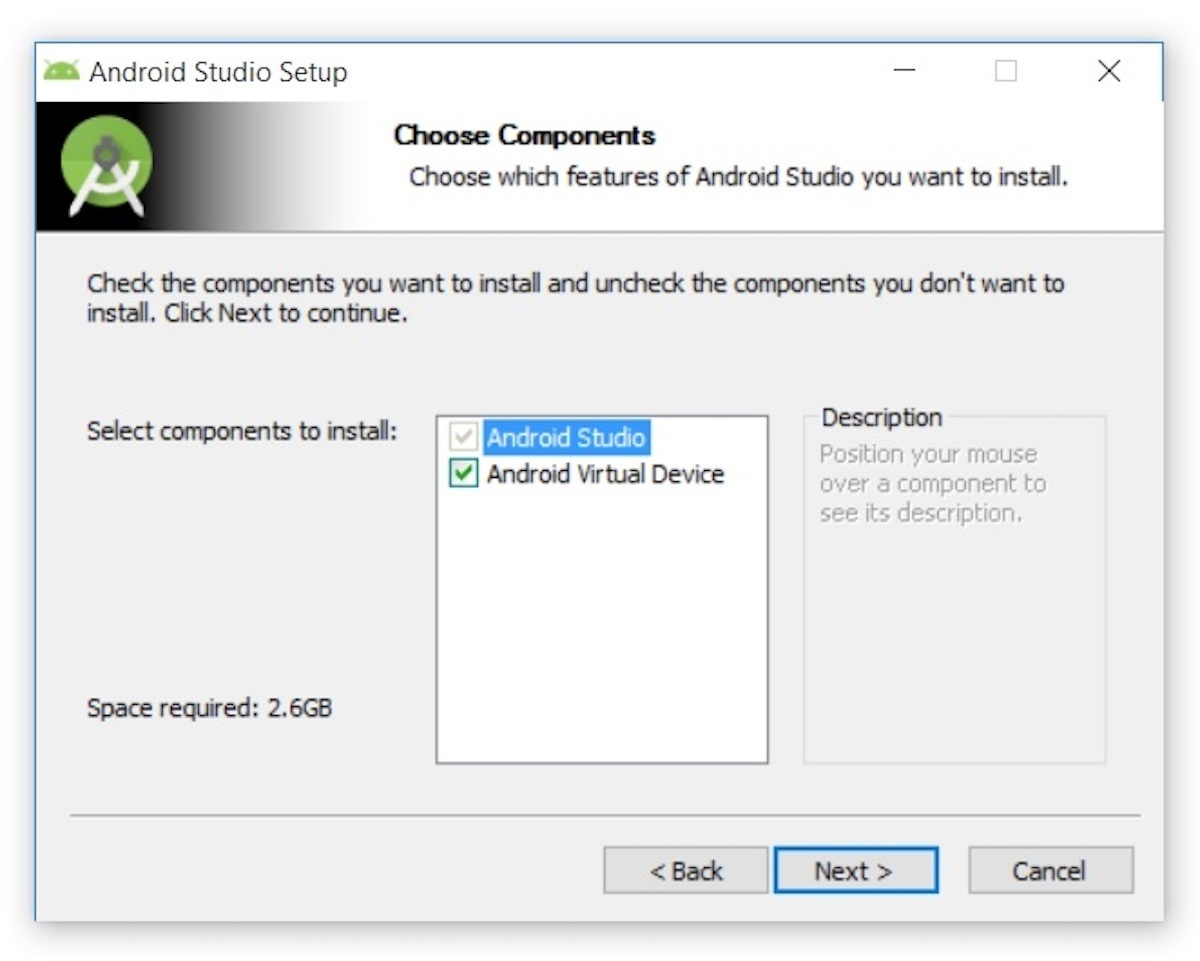
\includegraphics[width=4cm]{figures/installas/2.jpg}
		\centering
		\caption{Instal Android AVD.}
	\end{figure}
	\item Kemudian kita diminta untuk memilih lokasi tempat menginstal Android Studio-nya. Disini kita biarkan default setting-nya, lalu klik Next.
	\begin{figure}[H]
		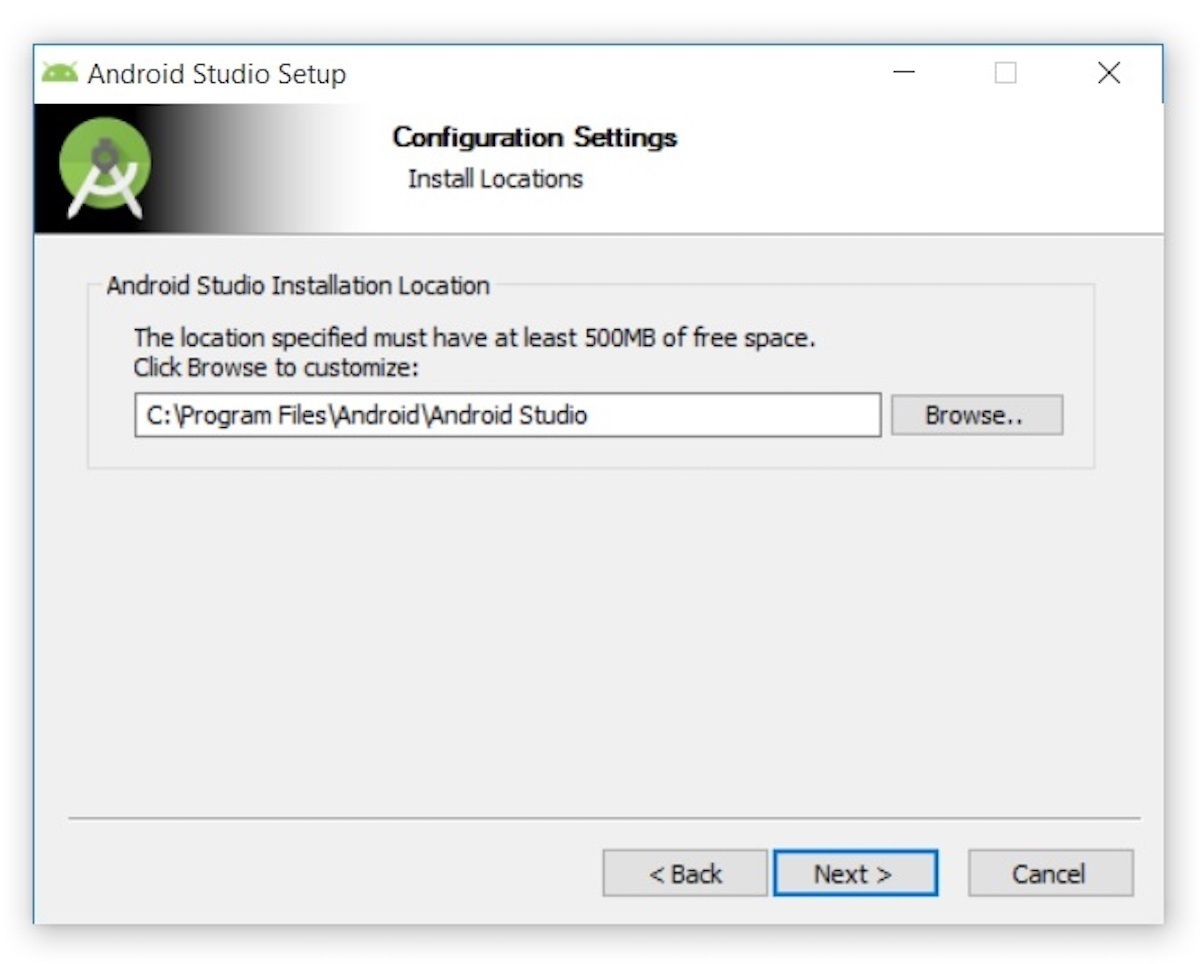
\includegraphics[width=4cm]{figures/installas/3.jpg}
		\centering
		\caption{Lokasi instal Android Studio.}
	\end{figure}
	\item Setelah itu, kita diberi opsi untuk membuat shortcut dari Android Studio. Disini kita biarkan default setting-nya, lalu klik Install.
	\begin{figure}[H]
		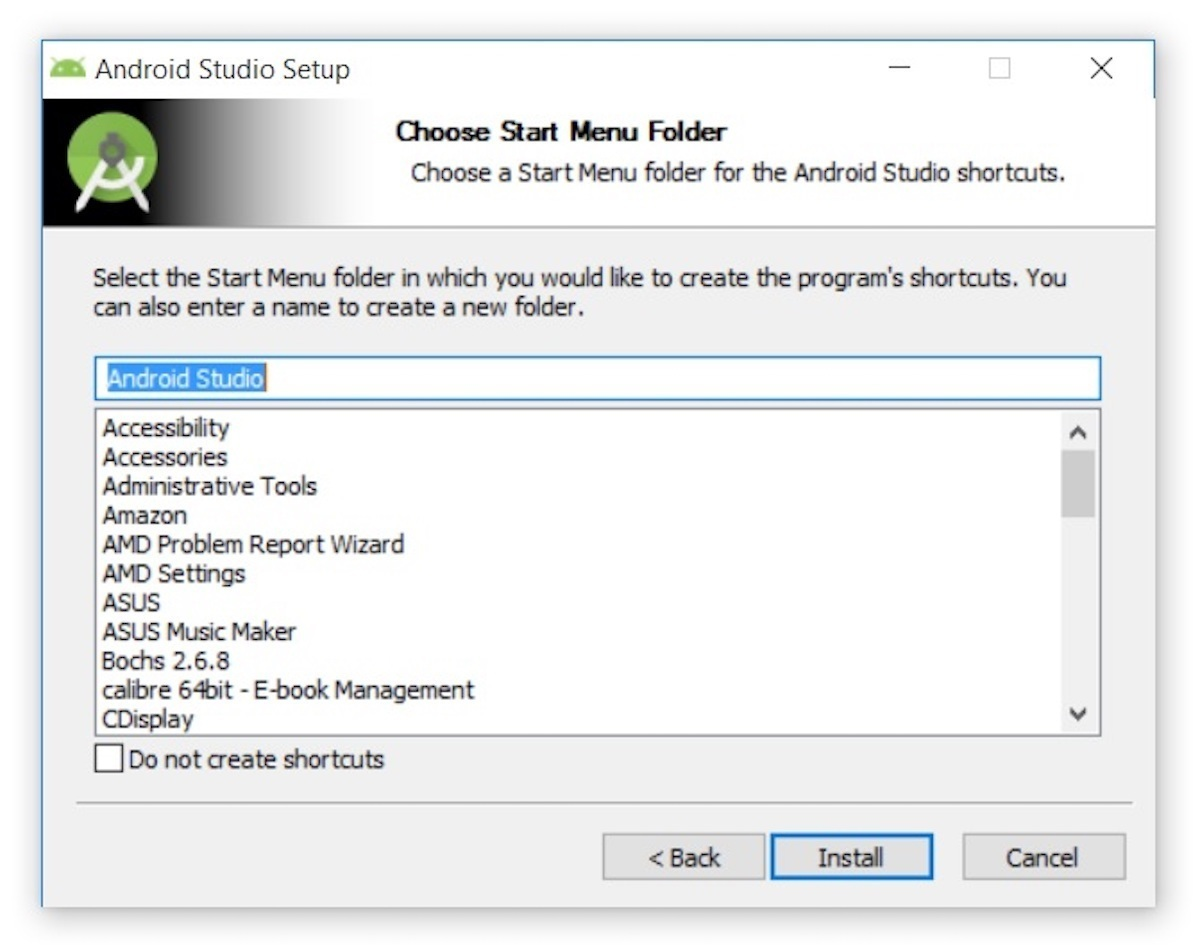
\includegraphics[width=4cm]{figures/installas/4.jpg}
		\centering
		\caption{Membuat shorcut Android Studio.}
	\end{figure}
	\item Kemudian proses instalasi akan berjalan. Show details untuk menampilkan file yang diinstal.
	\begin{figure}[H]
		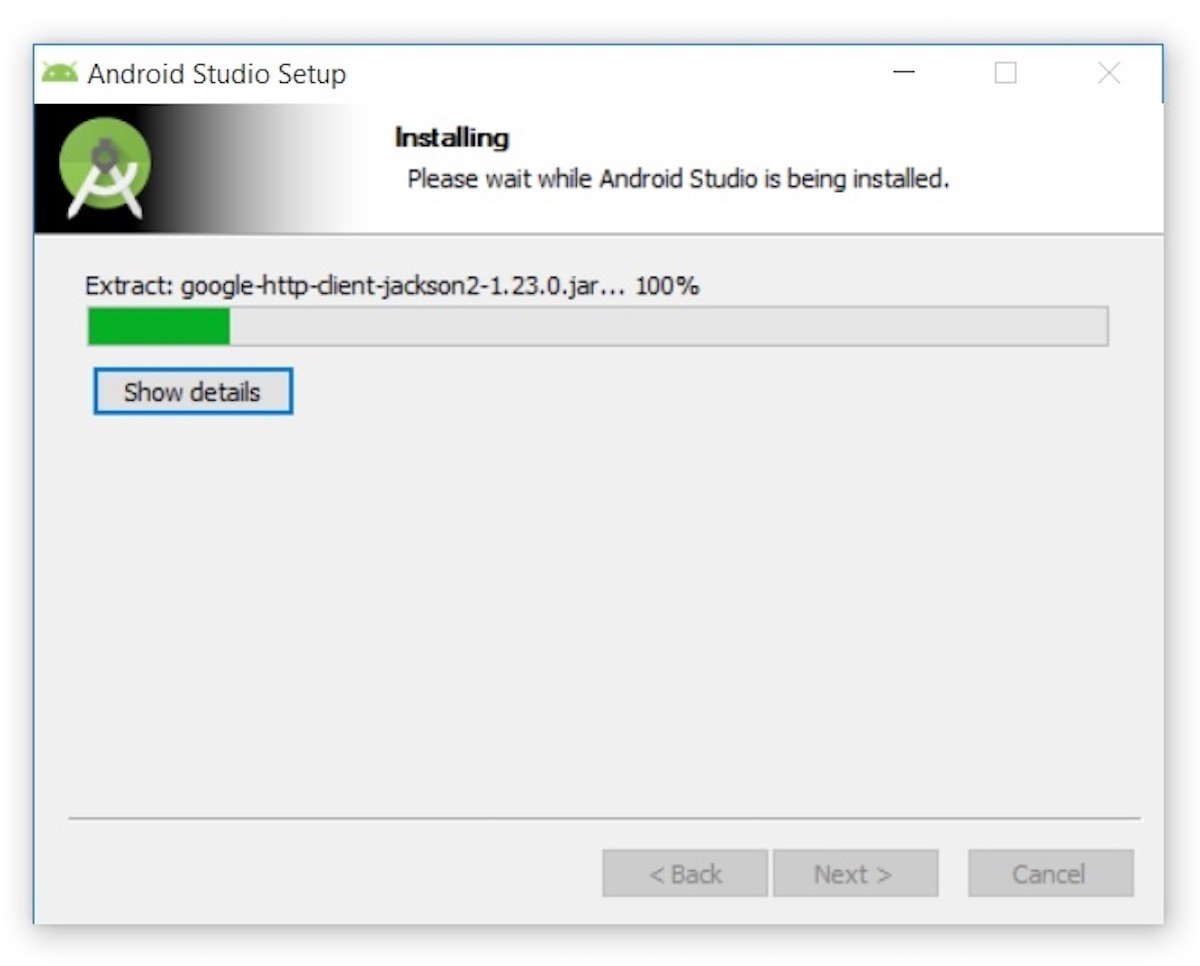
\includegraphics[width=4cm]{figures/installas/5.jpg}
		\centering
		\caption{Proses instalasi.}
	\end{figure}
	\item Setelah proses instal selesai, klik Next.
	\begin{figure}[H]
		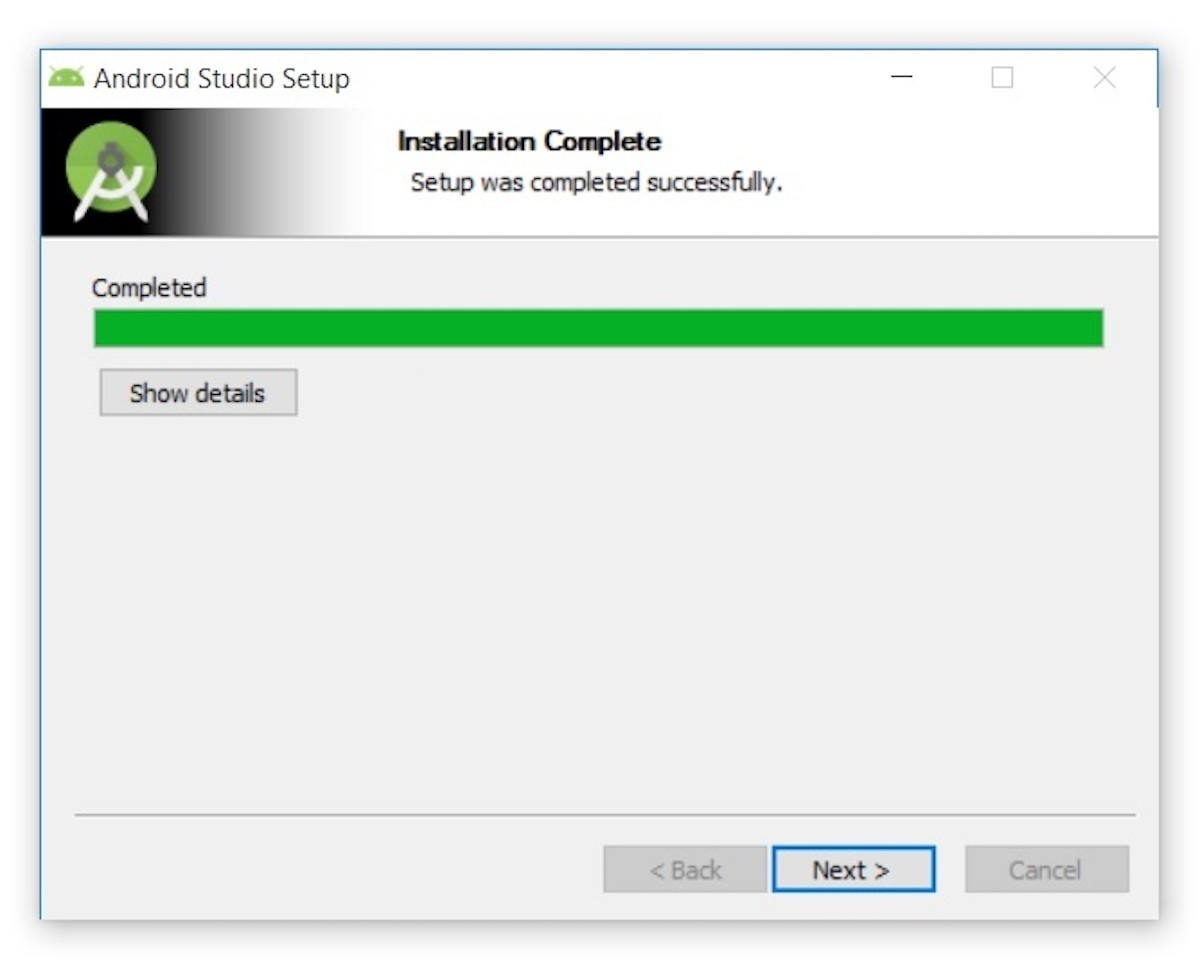
\includegraphics[width=4cm]{figures/installas/6.jpg}
		\centering
		\caption{Proses instalasi selesai.}
	\end{figure}
	\item Kemudian centang Start Android Studio untuk membuka aplikasinya, lalu klik Finish.
	\begin{figure}[H]
		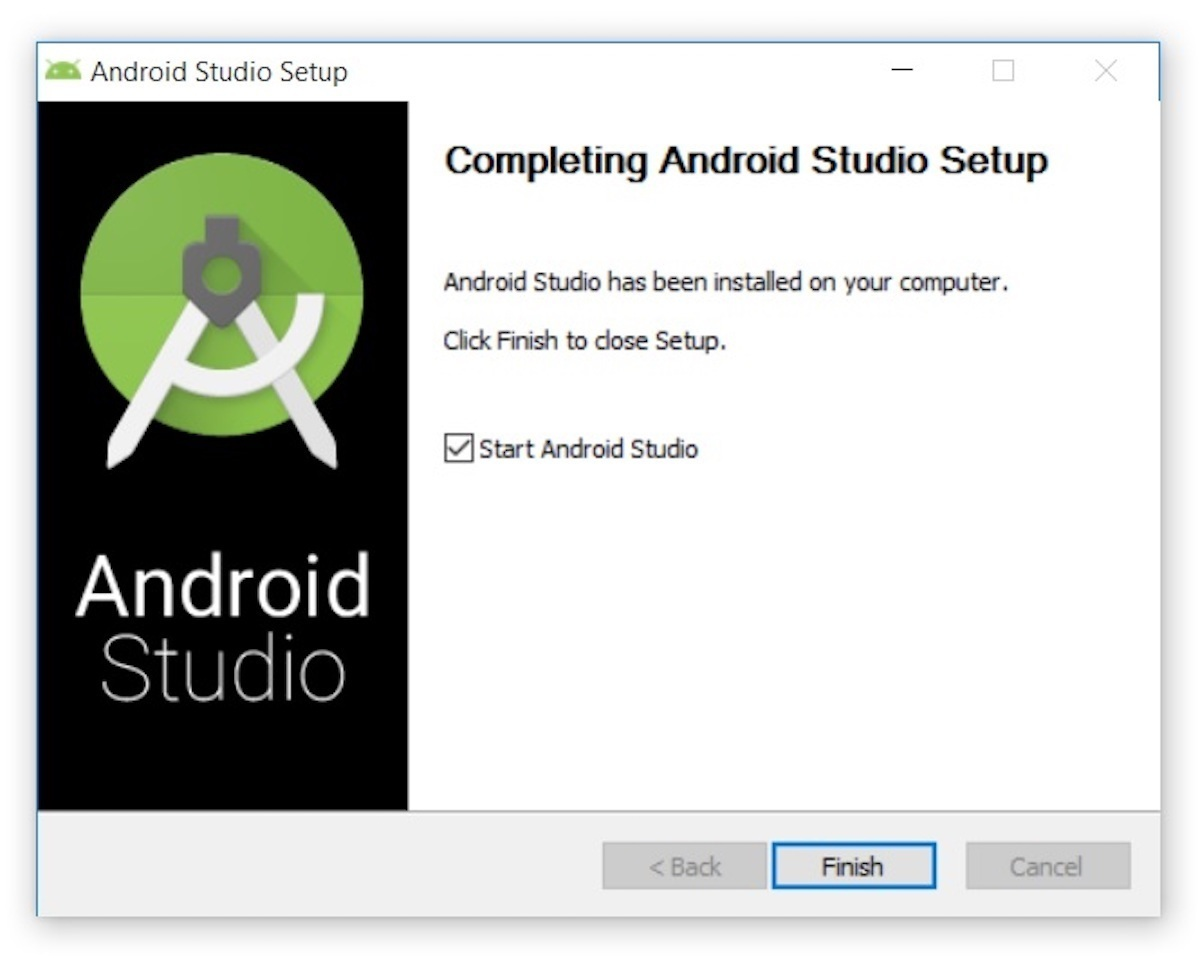
\includegraphics[width=4cm]{figures/installas/7.jpg}
		\centering
		\caption{Jalankan Android Studio.}
	\end{figure}
	\item Ketika Android Studio dijalankan pertama kali, dialog Complete Installation akan muncul dan memberi opsi untuk mengimport setting dari instalasi sebelumnya. Disini kita pilih Do not import settings, lalu klik OK.
	\begin{figure}[H]
		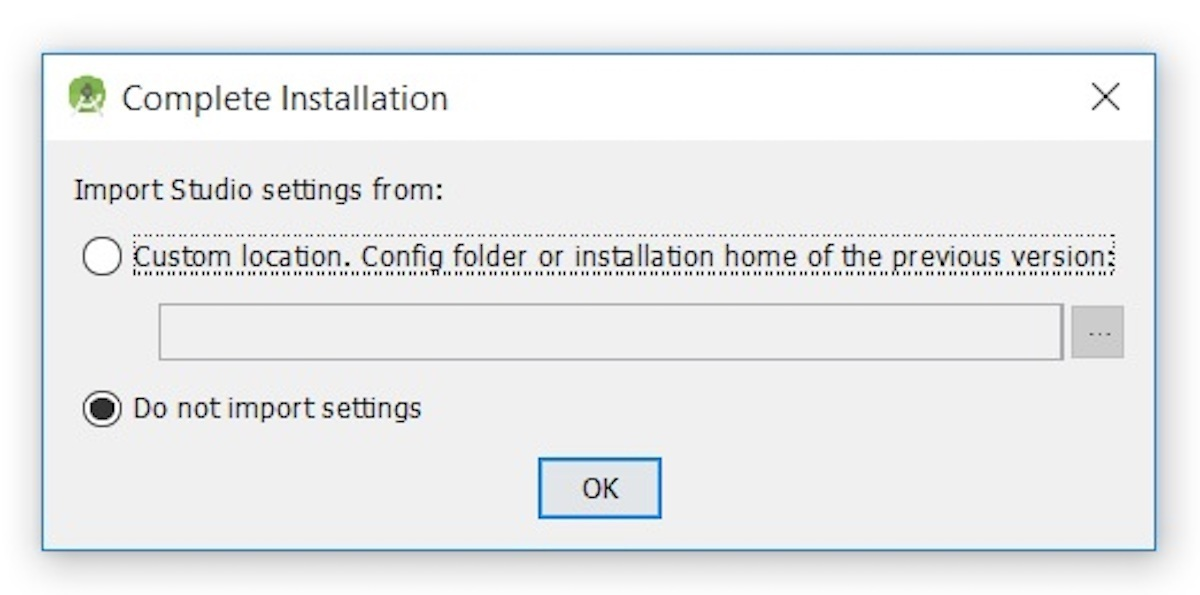
\includegraphics[width=4cm]{figures/installas/8.jpg}
		\centering
		\caption{Import setting instalasi sebelumnya.}
	\end{figure}
	
	\item Kemudian akan muncul splash screen dari Android Studio.
	\begin{figure}[H]
		
\includegraphics[width=4cm]{figures/installas/9.jpg}
		\centering
		\caption{Splash screen Android Studio.}
	\end{figure}
	
	\item Pertama
	\begin{figure}[H]
		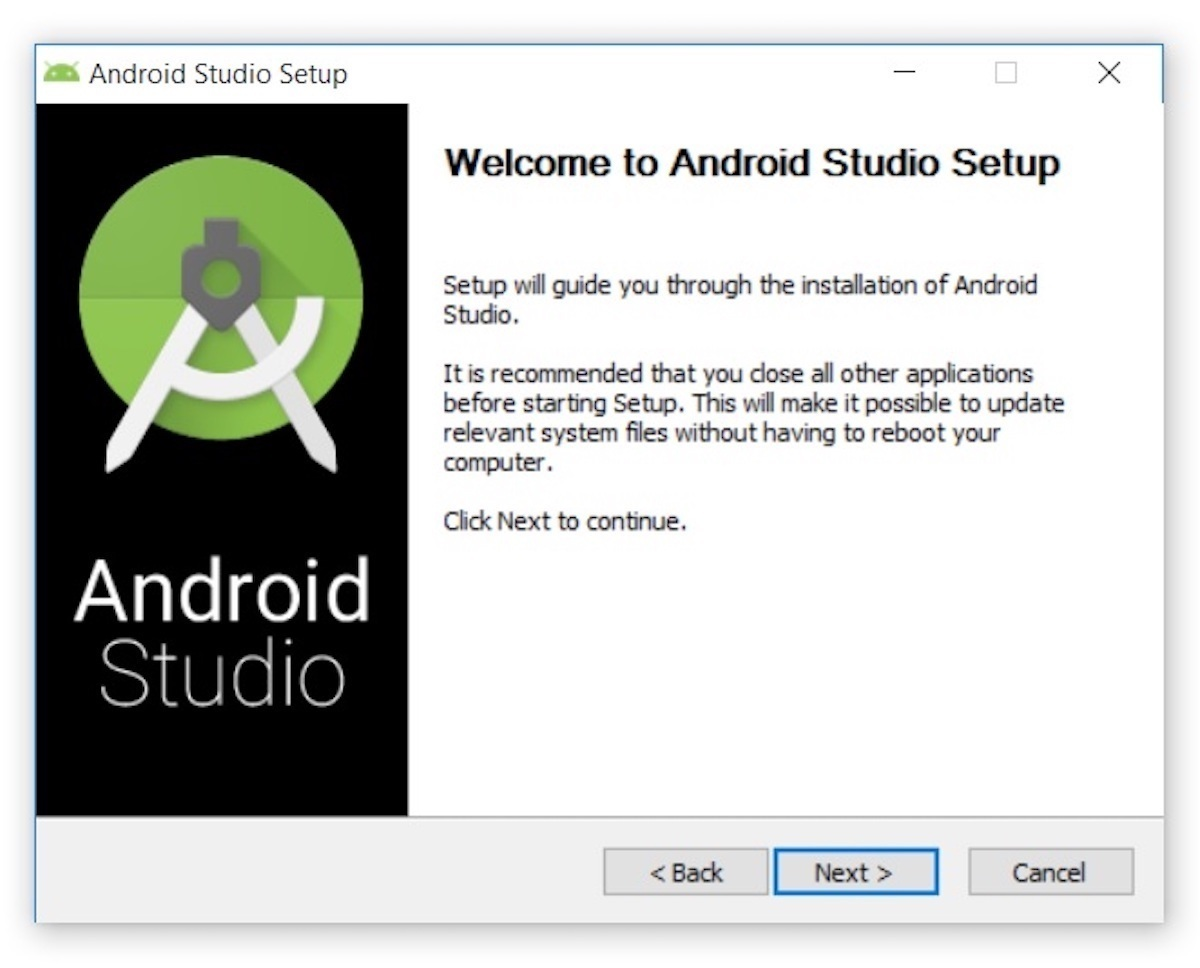
\includegraphics[width=4cm]{figures/installas/1.jpg}
		\centering
		\caption{.}
	\end{figure}
	
	\item Pertama
	\begin{figure}[H]
		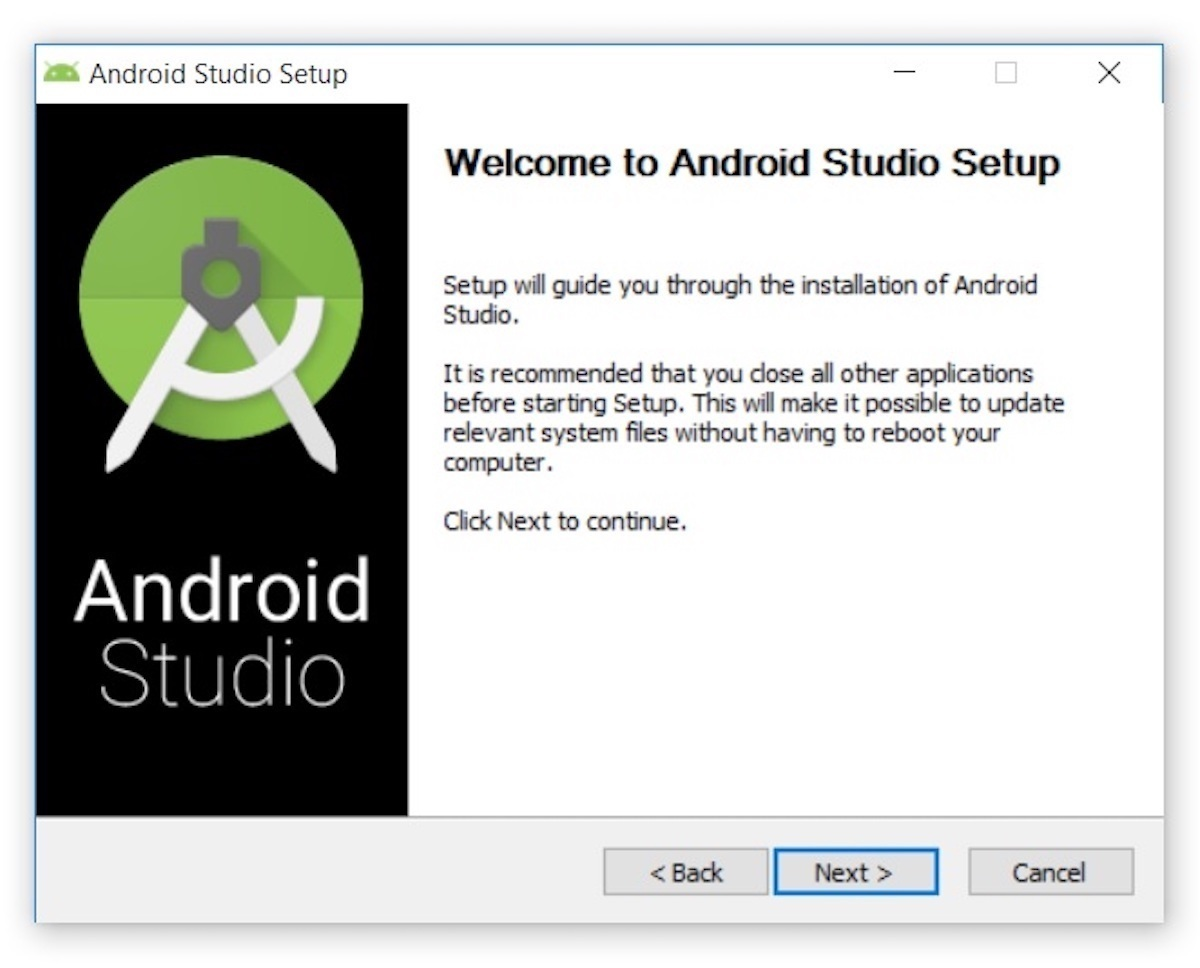
\includegraphics[width=4cm]{figures/installas/1.jpg}
		\centering
		\caption{.}
	\end{figure}
	
	\item Pertama
	\begin{figure}[H]
		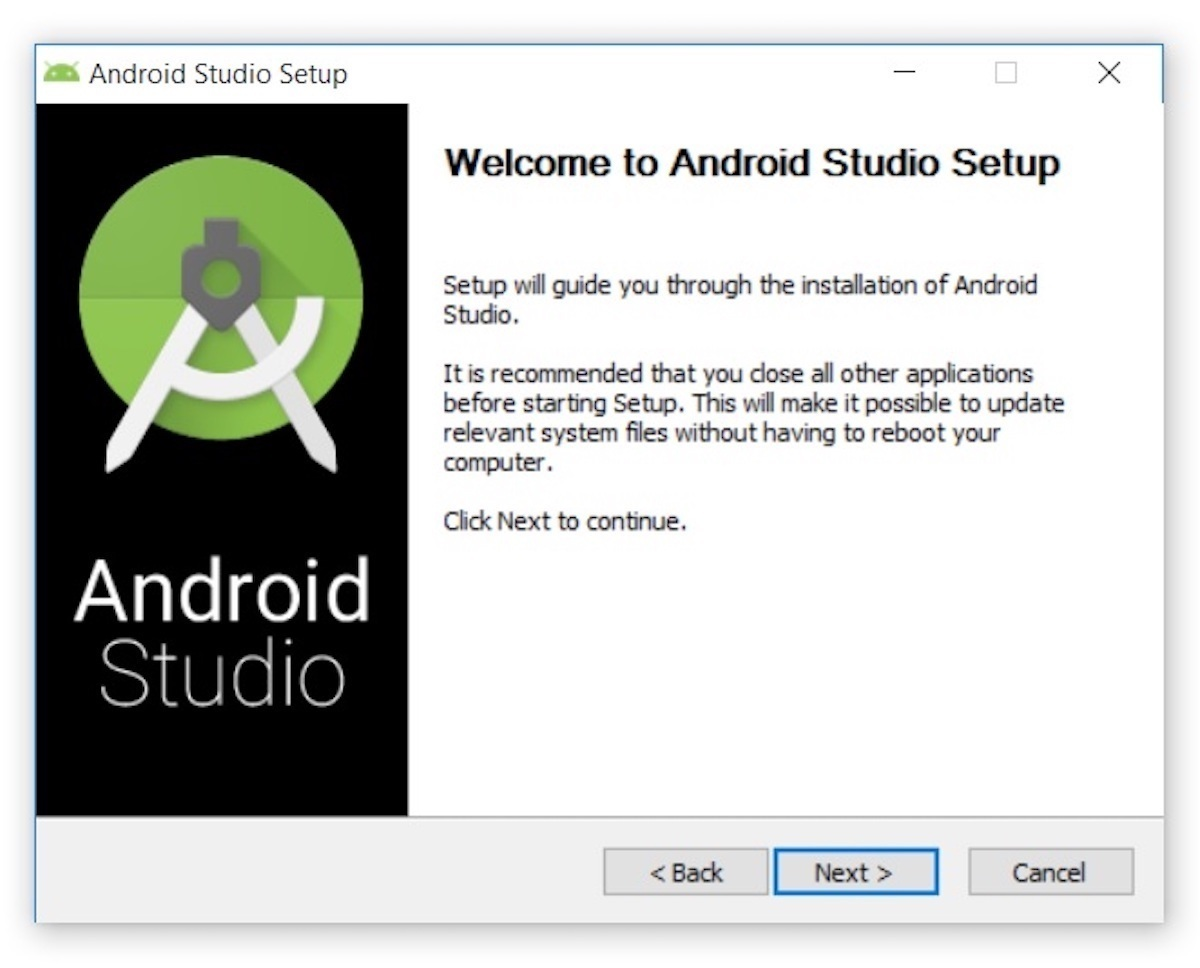
\includegraphics[width=4cm]{figures/installas/1.jpg}
		\centering
		\caption{.}
	\end{figure}
	
	\item Pertama
	\begin{figure}[H]
		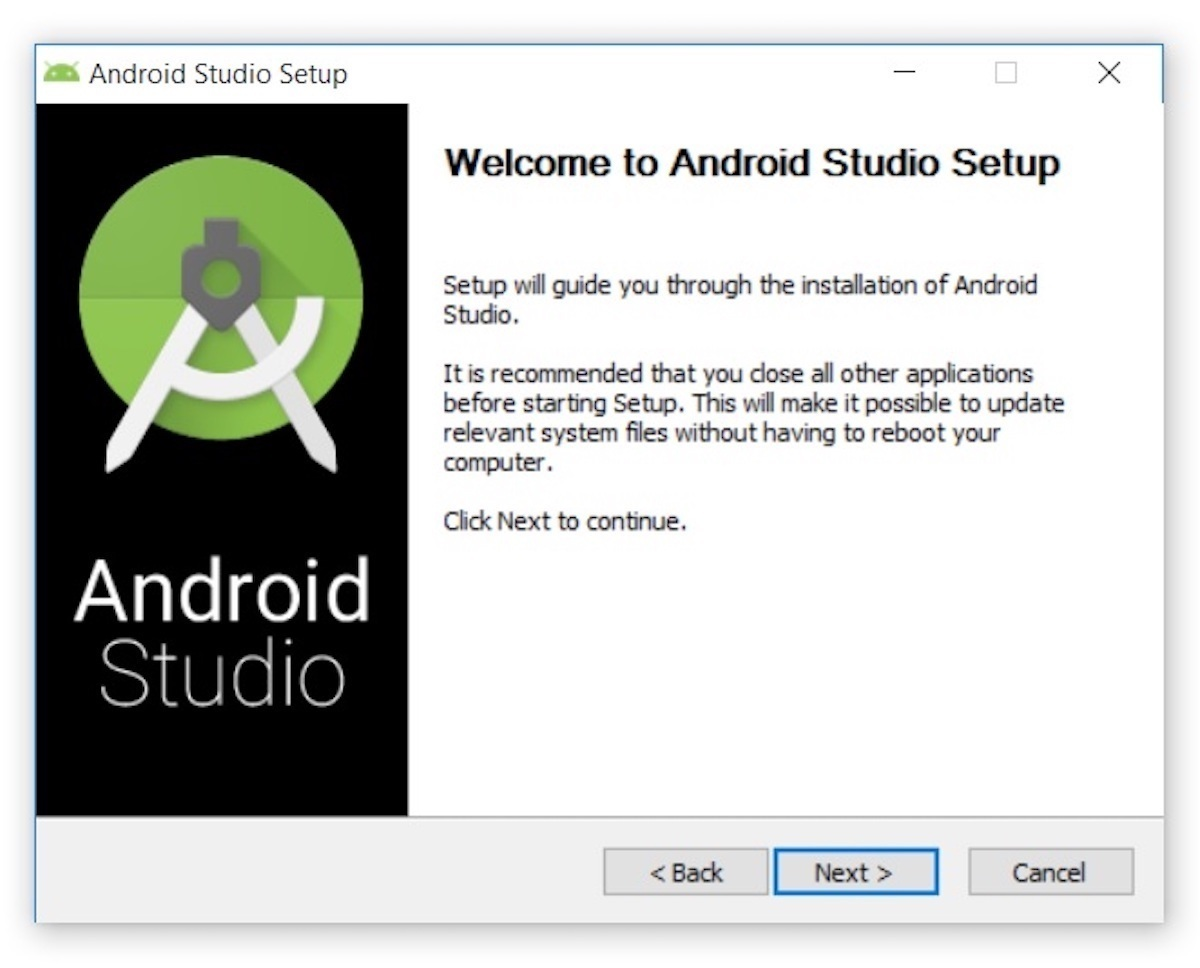
\includegraphics[width=4cm]{figures/installas/1.jpg}
		\centering
		\caption{.}
	\end{figure}
	
	\item Pertama
	\begin{figure}[H]
		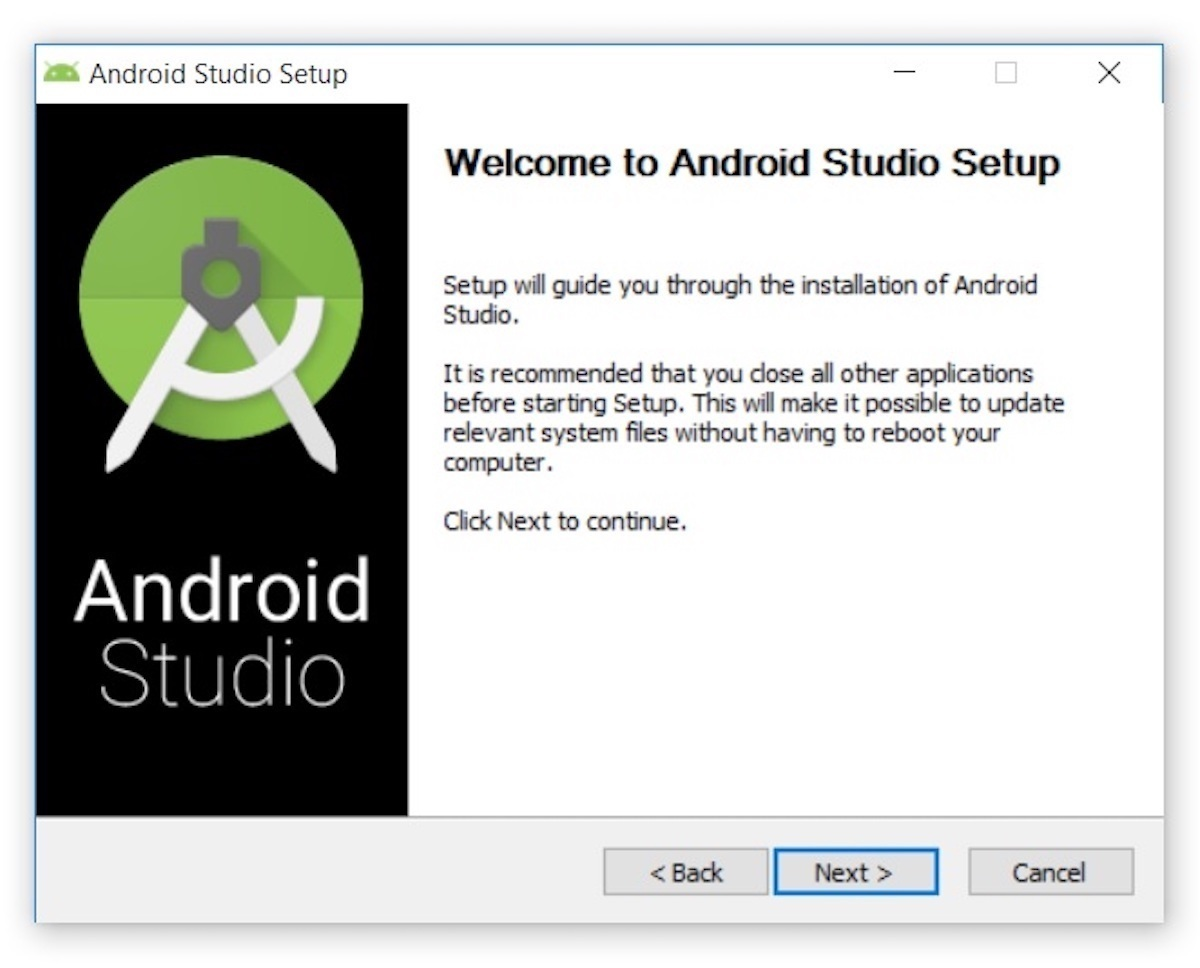
\includegraphics[width=4cm]{figures/installas/1.jpg}
		\centering
		\caption{.}
	\end{figure}
	
	\item Pertama
	\begin{figure}[H]
		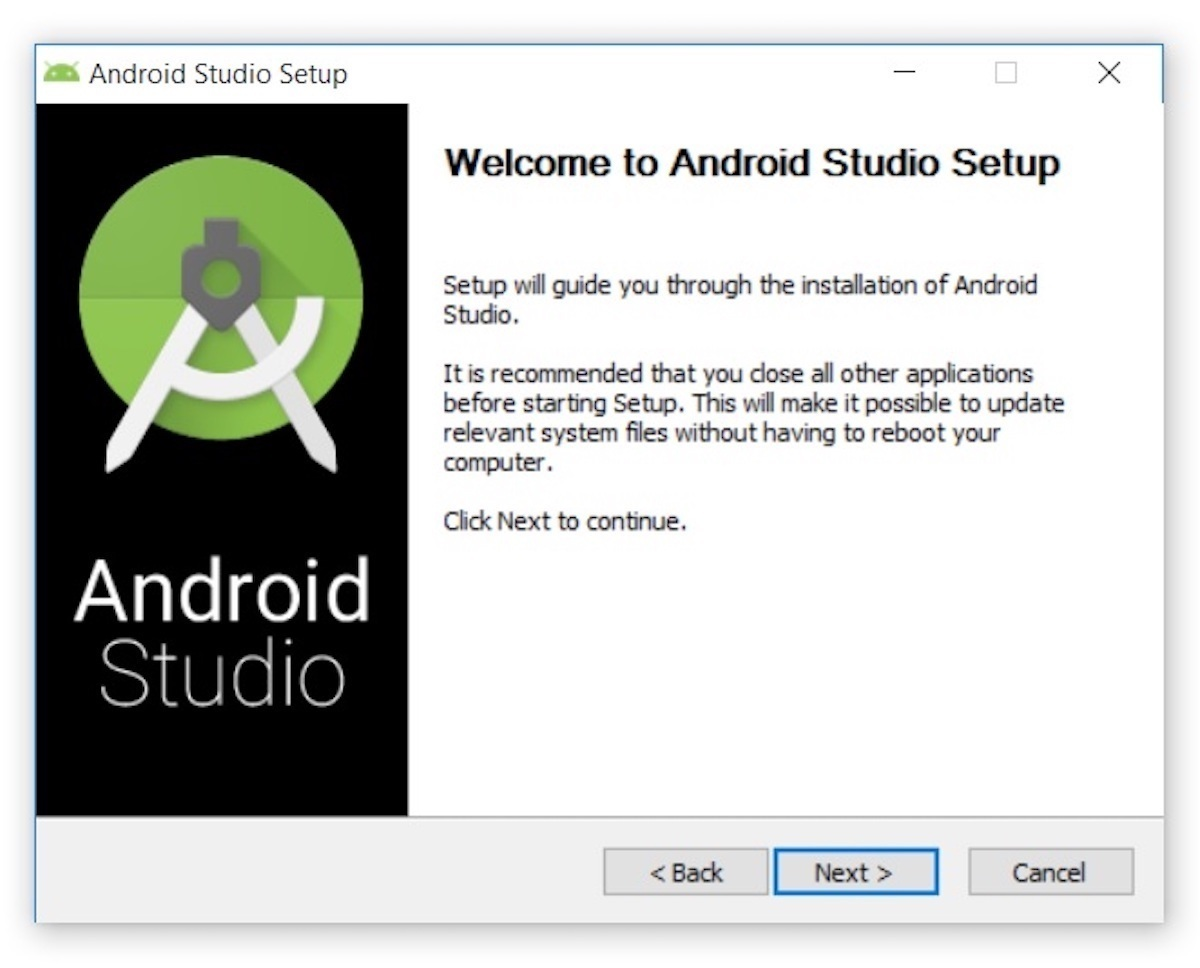
\includegraphics[width=4cm]{figures/installas/1.jpg}
		\centering
		\caption{.}
	\end{figure}
	
\end{enumerate}